\documentclass[a4paper,12pt]{article}

% paquets pour avoir les lettres accentués et la typographie française
\usepackage{a4wide}
\usepackage[utf8]{inputenc}
\usepackage[frenchb]{babel}

%\usepackage{glossaries}



\usepackage[colorlinks=true,linkcolor=black]{hyperref}
\usepackage[T1]{fontenc}%la police utilisee dans le document

%trois package pour taper du texte mathémathiques
\usepackage{amsmath}
\usepackage{amssymb}
\usepackage{amsfonts}
\usepackage{mathrsfs}

%pour insérer des styles de liste supplémentaire
%\usepackage{enumerate}

%pour l'insertion d'image
\usepackage{graphicx}
\usepackage{float}% pour l'utilisation de "centering" et de l'option [H] qui permet de placer plus efficacement les images

%package pour les lien url :
\usepackage{url}


%pour l'insertion de code source


\usepackage{fancyvrb}

\begin{document}

%%%%%%%%%%%%%%%%%%%%%%%%%%%%%%%%%%%%%%%%%%%%%%%%%%%%
% PAGE DE GARDE
%%%%%%%%%%%%%%%%%%%%%%%%%%%%%%%%%%%%%%%%%%%%%%%%%%%%

\begin{titlepage}
\begin{flushleft}
\large{Universit\'e du Havre \\
Master Matis \\
Sp\'ecialisation SIRES\\
}
\end{flushleft}

\setlength{\parskip}{96pt}

\begin{center}
\huge\textbf{TeXloud\\Des documents \LaTeX ~dans le Cloud}

\setlength{\parskip}{18pt}
\large\textsc{Référent: Y. Pigné}

\setlength{\parskip}{70pt}

\Large\textbf{Cahier des charges}

\setlength{\parskip}{50pt}

\large Adrien Bruyère\\David Ducatel\\Meva Rakotondratsima\\Sidina Biha\\Zakaria Bouchakor
\end{center}
\setlength{\parskip}{50pt}
\begin{flushleft}
\rule{.4mm}{26mm}\rule{105mm}{.4mm}
\today
\end{flushleft}
\end{titlepage}

%%%%%%%%%%%%%%%%%%%%%%%%%%%%%%%%%%%%%%%%%%%%%%%%%%%%
% FIN DE LA PAGE DE GARDE
%%%%%%%%%%%%%%%%%%%%%%%%%%%%%%%%%%%%%%%%%%%%%%%%%%%%
 
\clearpage

\tableofcontents

\newpage

\section{Introduction}
\paragraph*{}
LaTeX est un langage de composition de documents créé en 1983, dédié principalement à la rédaction
 de documents scientifiques, dont les éléments sémantiques sont définis par des mots-clés 
(définition de paragraphes, titres...). Il permet d'écrire simplement des formules scientifiques 
(équations mathématiques), et l'organisation des documents est gérée automatiquement (pagination, 
etc.).

\paragraph*{}
Le cloud computing repose sur le principe de délocalisation des traitements informatiques
 traditionnellement localisés sur des serveurs locaux ou sur le poste client de l'utilisateur. Cela 
permet une meilleure répartition des charges systèmes et des tâches.

\section{Description de la demande}

\subsection{Produit du projet}
 	
\paragraph*{} 
Ce projet propose la création et la gestion collaborative de documents
Latex. Le but est de proposer à des plateformes dépourvues de distribution
Latex (tablettes, smartphones, desktops), de se connecter au Web et
d’accéder à ces service de gestion et de compilation de documents.
\paragraph*{} 
Les utilisateurs seront authentifiés au service et bénéficieront d’un espace
de stockage privé. L'applications facilitera le partage de documents et le
travail collaboratif entre utilisateurs du service.
\paragraph*{} 
Coté client, deux types d'applications seront développés :\\

\begin{itemize}
 \item Un service Web permettra l’accès au service à partir de n’importe
quelle machine (desktop, tablette non-Android) pourvue d’un navigateur
Web et d’une connexion internet

 \item Une application Android, permettra une certaine autonomie avec le
stockage temporaire d’une copie de travail des documents, permettant
un mode d’édition non-connecté.
\end{itemize}
\newpage
\subsection{Les fonctions du produit}
 	
Les fonctionnalités principales du produit sont les suivantes :\\

\begin{itemize}
 \item FP0 - \'Edition des documents Latex
 \item FP1 - Accès à l'ensemble des projets
 \item FP2 - Interface Web et Android
 \item FP3 - Compilation Latex
 \item FP4 - Création de compte
 \item FP5 - Authentification
 \item FP6 - Téléchargement des documents
 \item FP7 - Synchronisation des documents
 \item FP8 - Charte graphique
\end{itemize}
\bigskip
Fonctionnalités complémentaires :\\
\begin{itemize}
 \item FC0 - Versioning (gestion de conflits, etc.)
 \item FC1 - Gestion des groupes d'utilisateurs
 \item FC2 - Gestion des erreurs
 \item FC3 - Unification des interfaces
 \item FC4 - Sauvegarde locale (travail offline)
\end{itemize}

\paragraph{FP0 - \'Edition des documents Latex\\}
La fonctionnalité principale de l'interface (Android ou Web) est l'édition de documents Latex. 
L'éditeur sera la zone principale de l'application, afin de pouvoir afficher le plus de texte 
possible.

\paragraph{FP1 - Accès à l'ensemble des projets\\}
Lors de l'authentification, l'utilisateur récupère l'arborescence de ses projets (dossiers, 
fichiers). Le fichier sélectionné sera ensuite téléchargé, et l'utilisateur pourra travailler.

\paragraph{FP2 - Interface Web et Android\\}
L'utilisateur a deux possibilités pour se connecter à TeXloud, \emph{via} :\\
\begin{itemize}
 \item Interface web : on peut se connecter de n'importe quel poste (ordinateur personnel, cybercafé...)
 \item Système Android : connexion à partir d'une tablette Android. L'utilisateur pourra alors 
travailler par un réseau Wifi ou 3G, ou bien en local (offline).
\end{itemize}

\paragraph{FP3 - Compilation Latex\\}
Lorsque l'utilisateur souhaite avoir un rendu PDF de son document Latex, il doit pouvoir demander 
la compilation au serveur.

\paragraph{FP4 - Création de compte\\}
Pour qu'un utilisateur puisse utiliser le service TeXloud, une inscription est nécessaire. La 
création de compte est faisable par l'application android ou l'application web. L'utilisateur doit
fournir un nom, un mot de passe et une adresse mail.

\paragraph{FP5 - Authentification\\}
A chaque démarrage de l'application, l'utilisateur envoie son login et mot de passe. L'authentification
est nécessaire pour pouvoir utiliser l'application TeXloud.

\paragraph{FP6 - Téléchargement des documents\\}
Le téléchargement des documents est une fonctionnalité capitale de l'application. Les documents 
compilés (PDF) doivent pouvoir être envoyés à l'utilisateur, ainsi que les fichiers Latex, pour que 
l'utilisateur travaille toujours sur la version la plus récente.

\paragraph{FP7 - Synchronisation des documents\\}
Un fichier Latex en cours de modification doit être régulièrement synchronisé avec le serveur.

\paragraph{FP8 - Charte graphique\\}
Définir une charte graphique.


\paragraph{FC0 - Versioning (gestion de conflits, etc.)\\}
L'application devra intégrer un gestionnaire de version, afin de permettre un meilleur travail de
groupe.

\paragraph{FC1 - Gestion des groupes d'utilisateurs\\}
Plusieurs personnes peuvent travailler sur un même projet. Chaque projet a donc un ou plusieurs 
utilisateurs qui ont le droit de modifier les fichiers. Le créateur du projet doit former le groupe.

\paragraph{FC2 - Gestion des erreurs\\}
Le client doit pouvoir voir les différentes erreurs, afin de les corriger. Par exemple : erreur 
de compilation, conflit de version sur un fichier.

\paragraph{FC3 - Unification des interfaces\\}
L'interface des deux applications doit être similaire. L'utilisateur doit pouvoir retrouver ses
repères rapidement, en passant d'une application à l'autre. Par exemple : position et ordre des 
éléments, onglets, thème graphique.

\paragraph{FC4 - Sauvegarde locale (travail offline)\\}
Une tablette Android peut à tout moment perdre sa connexion Internet (voyage, zone non couverte). 
Il est donc important de pouvoir travailler hors-ligne à partir d'un fichier temporaire.

\newpage
\subsection{Infrastructure physique}

\begin{figure}[!ht]
\begin{center}
  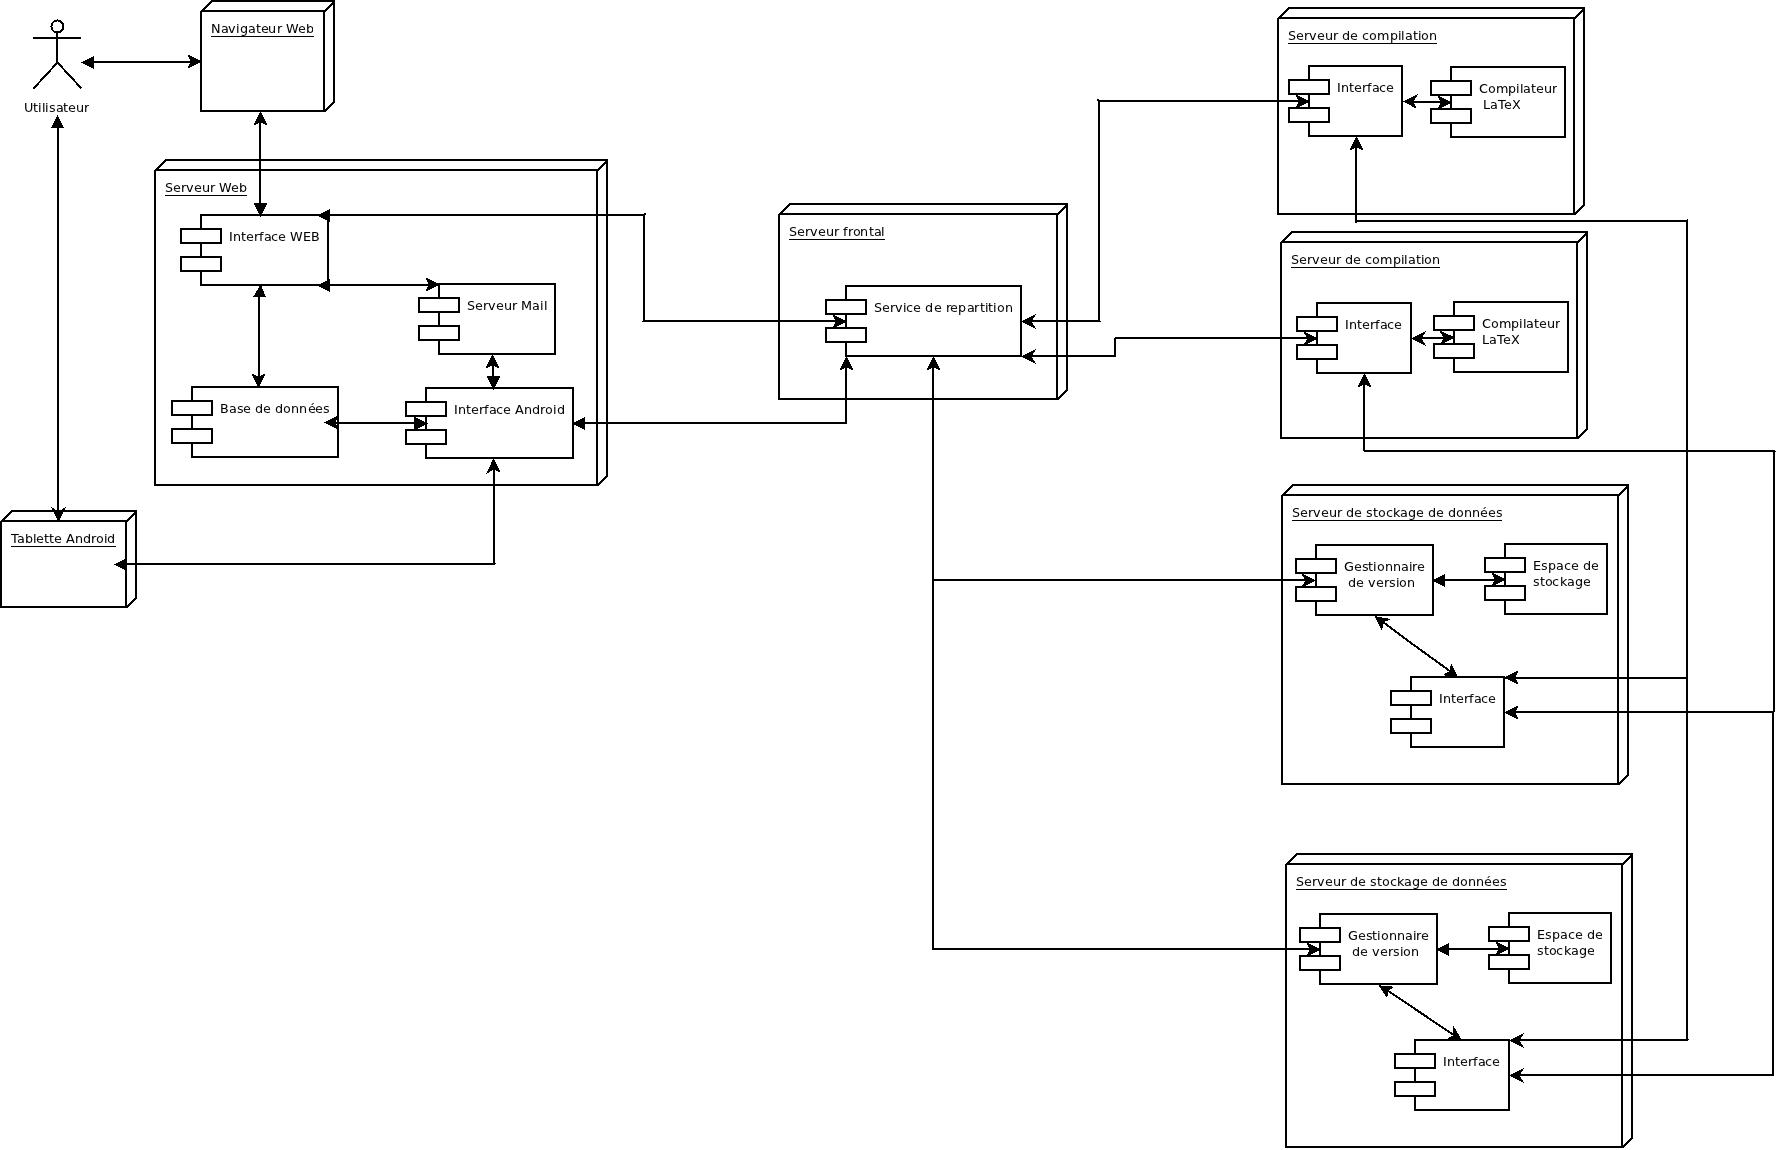
\includegraphics[width=1\textwidth,angle=90]{./Diagramme/DiagrammeDeploiement.jpg}
\end{center}
  \caption{Diagramme de déploiement}
  \label{déploiement}
\end{figure}
\newpage




%\subsection{Critères d'acceptabilité et de réception}
 	
%Le projet pourra être considéré comme complet, si les critères ci-dessous sont remplis :
%\begin{itemize}
% \item L'interface web est entièrement développée en HTML5 et validée par le W3C
% \item Les services de compilation et de stockage de données sont distribués sur plusieurs machines
% \item Les interfaces Android et Web sont unifiées
% \item L'application est utilisable
%\end{itemize}


\section{Contraintes}

\subsection{Contrainte de délais}

Audits intermédiaires :
\begin{itemize}
 \item 09 Décembre 2011
 \item 06 Janvier 2012
 \item 13 Janvier 2012
\end{itemize}

Rendu de projet : Courant Février 2012

\subsection{Contraintes technique}
 	
\paragraph*{}
Les données devront pouvoir être stocké sur un ou plusieurs serveurs avec un support de plusieurs logiciel de versioning (GIT,SVN).

\paragraph*{}
La compilation des documents latex devra être possible sur un ou plusieurs serveurs.

\paragraph*{}
La visualisation des documents PDF devra être effectué dans un canvas HTML5 (génération entièrement en javascript).

\section{Déroulement du projet}

\subsection{Planification}
\newpage
\subsubsection{Diagramme de planification}
\begin{figure}[!ht]
\begin {center}
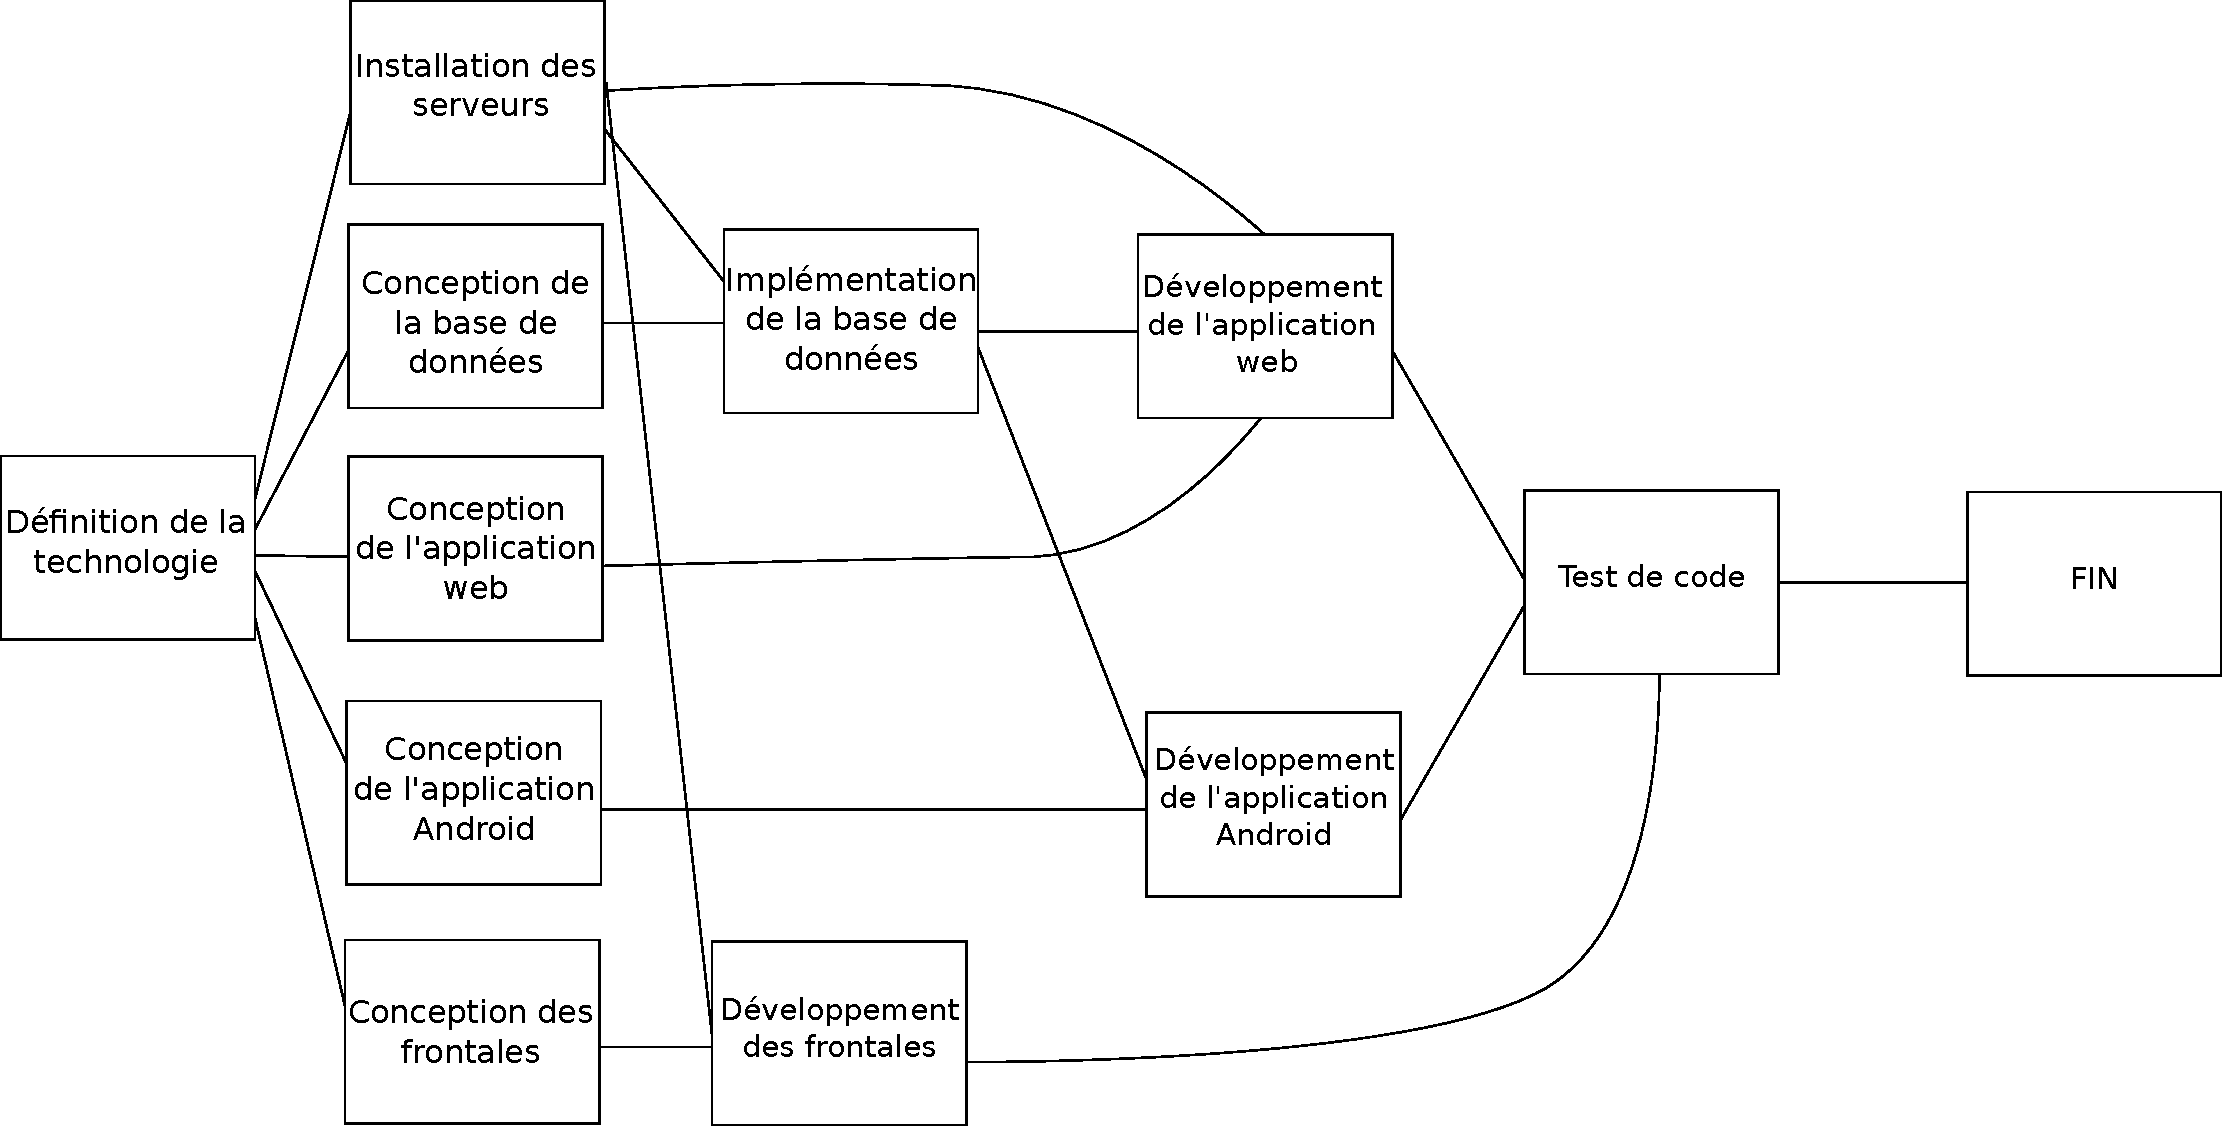
\includegraphics[width=1\textwidth,angle=90]{./Diagramme/mpm.pdf}
\end{center}
\label{MPM}
\caption{Diagramme de planification}
\end{figure}
\newpage

\subsubsection{Définition de l'environnement de développement}

\paragraph*{Environnement matériel\\} 
Nous avons besoin de 7 serveurs (virtualisation possible) et une tablette Android. Les serveurs sont :
\begin{itemize}
 \item Serveur Web, bases de données et mail
 \item Serveur frontal de gestion de données
 \item Deux serveurs de stockage des données
 \item Serveur frontal de compilation
 \item Deux serveurs de compilation
\end{itemize}


\paragraph*{Environnement logiciel\\}
\label{envlogiciel}
Voici les environnements logiciels utilisés :
\begin{itemize}
 \item Serveur http : Apache
 \item SGBD : PostgreSQL
 \item GIT et SVN pour le versioning et stockage de données
 \item Interpréteur PHP 5  
 \item Compilateur Latex
 \item Serveur SMTP Postfix
 \item Hyperviseur (si virtualisation)
 \item Système d'exploitation Android
\end{itemize}
 

\paragraph*{Langages de programmation\\}
Liste des langages de programmation utilisés pour la partie Web:
\begin{itemize}
 \item HTML 5, CSS 3
 \item PHP 5
 \item Javascript (jQuery)
 \item SQL
\end{itemize}

\paragraph*{}
Langage de programmations utilisé pour le développement des frontales : \emph{python}

\paragraph*{}
Langage de programmations utilisé pour le développement de l'application Android : \emph{Java et XML }


\subsubsection{Installation de serveurs}
L'étape consiste à installer tout l'environnement logiciel cité précédemment (voir point \ref{envlogiciel} page \pageref{envlogiciel}). 

\subsubsection{Conception de la base de données}
L'étape consiste à concevoir les besoins de l'application au niveau du stockage relationnel. Cette conception sera réalisé à l'aide de la méthode de conception Merise.

\subsubsection{Conception de l'application web}
L'étape consiste à définir l'ensemble des actions possibles sur l'application web, les interactions entre ses actions et le déroulement de chacune de ses même actions. Cette conception sera réalisé à l'aide de la méthode de conception UML.

\subsubsection{Conception de l'application Android}
L'étape consiste à définir l'ensemble des actions possibles sur l'application Android (qui seront plus ou moins équivalent au action disponible sur la partie application web), les interactions entre ses actions et le déroulement de chacune de ses même actions. Cette conception sera réalisé à l'aide de la méthode de conception UML.

\subsubsection{Conception des frontales}
L'étape consiste à définir les transmissions possible entre les frontales, le serveur web et les serveurs du cloud (pour la compilation ou le stockage de données). Cette étape permettra aussi de définir le protocole de communication et d'encapsulation de données afin d'éliminé tout risque de conflit dans les communication réseau entre les différentes parties. Cette conception sera réalisé à l'aide de la méthode de conception UML.

\subsubsection{Implémentation de la base de données}
L'étape consiste à créer un script SQL permettant de d'implémenter la base de données en fonction de la conception de celle-ci.

\subsubsection{Développement des frontales}
L'étape consiste à développer un ensemble de script Python qui vont permettre les communication entre le serveur web et les serveurs du cloud (serveur de compilation ou de stockage de données).

\subsubsection{Développement de l'application web}
L'étape consiste à développer un ensemble de page HTML5/PHP permettant a l'utilisateur de travailler sur ces projets LaTeX et d’interagir avec les serveurs du cloud (serveur de compilation ou de stockage de données).

\subsubsection{Développement de l'application Android}


\subsubsection{Test du code}
L'étape consiste à tester tous les modules de l'application (application Android, application web, frontale) ensemble afin de valider le fonctionnement global du projet. Cette étape permettra de trouver et corriger 
les éventuels bug qui pourrais rester.

\subsection{Ressources}
\paragraph*{}
Ressources humaines : 5 étudiants.
\begin{itemize}
 \item Adrien Bruyère: développement d'application Android
 \item David Ducatel, Meva Rakotondratsima: développement des applications frontales
 \item Sidina Biha, Zakaria Bouchakor: développement de l'application WEB
\end{itemize}

\paragraph*{}
Ressources matérielles : Serveur, Tablette.

\subsection{Norme des trames de communication}
\paragraph*{}
Les trames de communication seront tous formaté en JSON. Ils auront tous un
attribut Label qui correspondra à la tache a effectuer avec cette trame.
Ci-dessous se trouve la liste exhaustive des trames:

\paragraph{Trame entre le serveur HTTP et le serveur frontal:}
\begin{itemize}
 \item label:create,username,projectName
 \item label:getProject,path,servDataIp,servDataPort
 \item label:compile,rootFile,path,servDataIp,servDataPort
 \item label:getFile,path,servDataIp,servDataPort
 \item label:deleteFile,path,servDataIp,servDataPort
 \item label:deleteProject,path,servDataIp,servDataPort
 \item label:sync,path,servDataIp,servDataPort,currentFile
\end{itemize}

\paragraph{Trame entre le serveur frontal et un serveur de données:}
\begin{itemize}
 \item label:create,username,projectName
 \item label:getProject,path, username, client
 \item label:compile,rootFile,path,servCompileIp,servCompilePort
 \item label:getFile,path, username, password
 \item label:deleteFile,path, username, password
 \item label:deleteProject,path
 \item label:sync,path,currentFile, username, password
\end{itemize}

\paragraph{Trame entre le serveur frontal et un serveur de compilation:}
\begin{itemize}
 \item label:endCompilation,servCompileIp,servCompilePort
\end{itemize}

\subsection{Scénario}
\subsubsection{Diagramme de cas d'utilisation}
Voir annexe \ref{useCases} page \ref{useCases}.

\subsubsection{Diagramme de séquence de l'interface web}

\paragraph{Inscription:\\}
Voir annexe \ref{register} page \ref{register}.

\paragraph{Suppression de compte:\\}
Voir annexe \ref{deleteAccount} page \ref{deleteAccount}.

\paragraph{Création d'un projet:\\}
Voir annexe \ref{createProject} page \ref{createProject}.

\paragraph{Compilation de documents:\\}
Voir annexe \ref{compile} page \ref{compile}.

\paragraph{Téléchargement de fichier:\\}
Voir annexe \ref{download} page \ref{download}.

\paragraph{Partage de projet:\\}
Voir annexe \ref{share} page \ref{share}.

\paragraph{Synchronisation de documents:\\}
Voir annexe \ref{sync} page \ref{sync}.

\paragraph{Visualisation d'un projet:\\}
Voir annexe \ref{view} page \ref{view}.

\paragraph{Suppression d'un projet:\\}
Voir annexe \ref{deleteAccount} page \ref{deleteAccount}.

\paragraph{Téléchargement d'un projet:\\}
Voir annexe \ref{downloadProject} page \ref{downloadProject}.

\subsubsection{Diagramme de séquence de l'application Android}

\paragraph{Inscription:\\}
Voir annexe \ref{androidRegister} page \ref{androidRegister}.

\paragraph{Suppression de compte:\\}
Voir annexe \ref{androidDeleteAccount} page \ref{androidDeleteAccount}.

\paragraph{Création de projet:\\}
Voir annexe \ref{androidCreateProject} page \ref{androidCreateProject}.

\paragraph{Compilation de documents:\\}
Voir annexe \ref{androidCompile} page \ref{androidCompile}.

\paragraph{Téléchargement de documents :\\}
Voir annexe \ref{androidDownload} page \ref{androidDownload}.

\paragraph{Suppression d'un projet:\\}
Voir annexe \ref{androidDel} page \ref{androidDel}.

\paragraph{Téléchargement d'un projet:\\}
Voir annexe \ref{androidDownloadProject} page \ref{androidDownloadProject}.


\subsection{Charte graphique}
\subsubsection{Page d'authentification}
\paragraph{}
\begin{figure}[!ht]
\begin{center}
  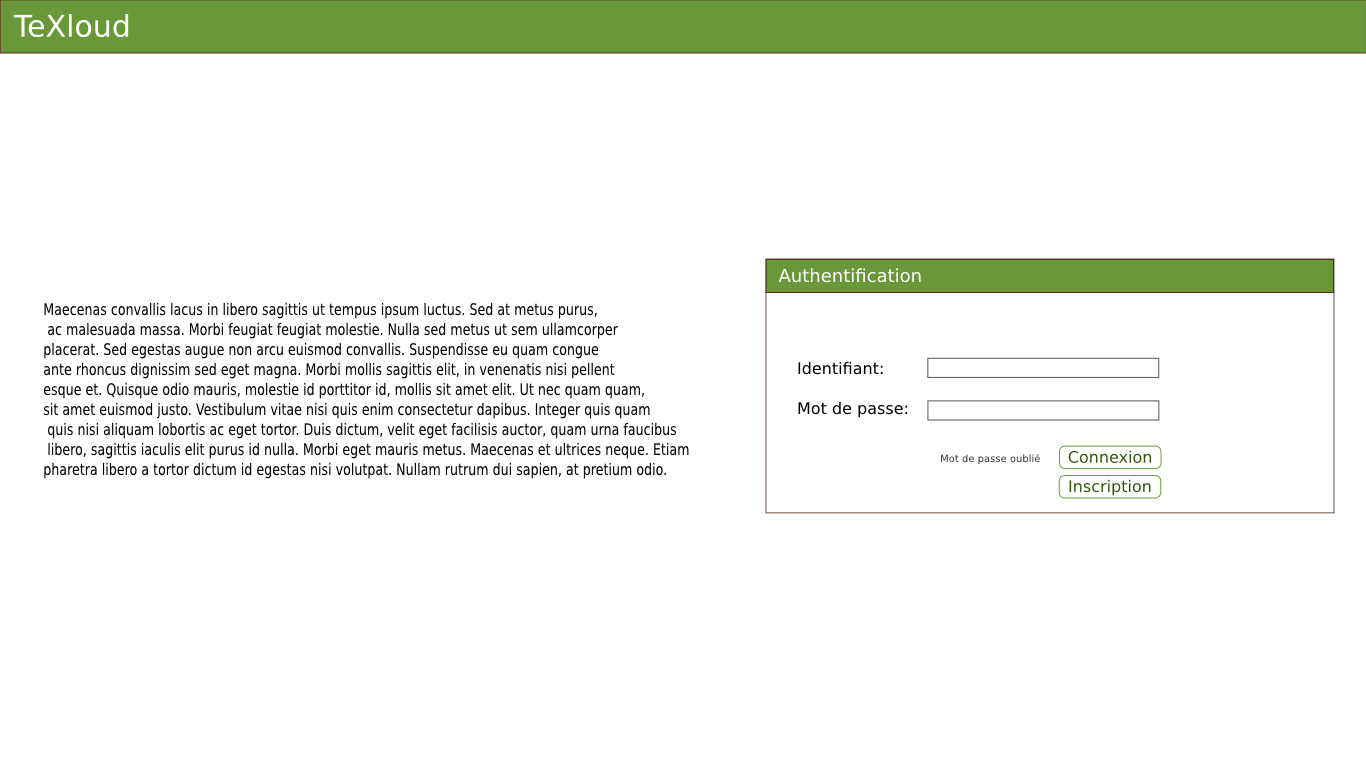
\includegraphics[width=1\textwidth, angle=90]{../layout/layout_texloud_login.png}
\end{center}
  \caption{Page d'authentification}
  \label{uiAuth}
\end{figure}

\newpage
\subsubsection{Interface de projet}
\paragraph{}
\begin{figure}[!ht]
\begin{center}
  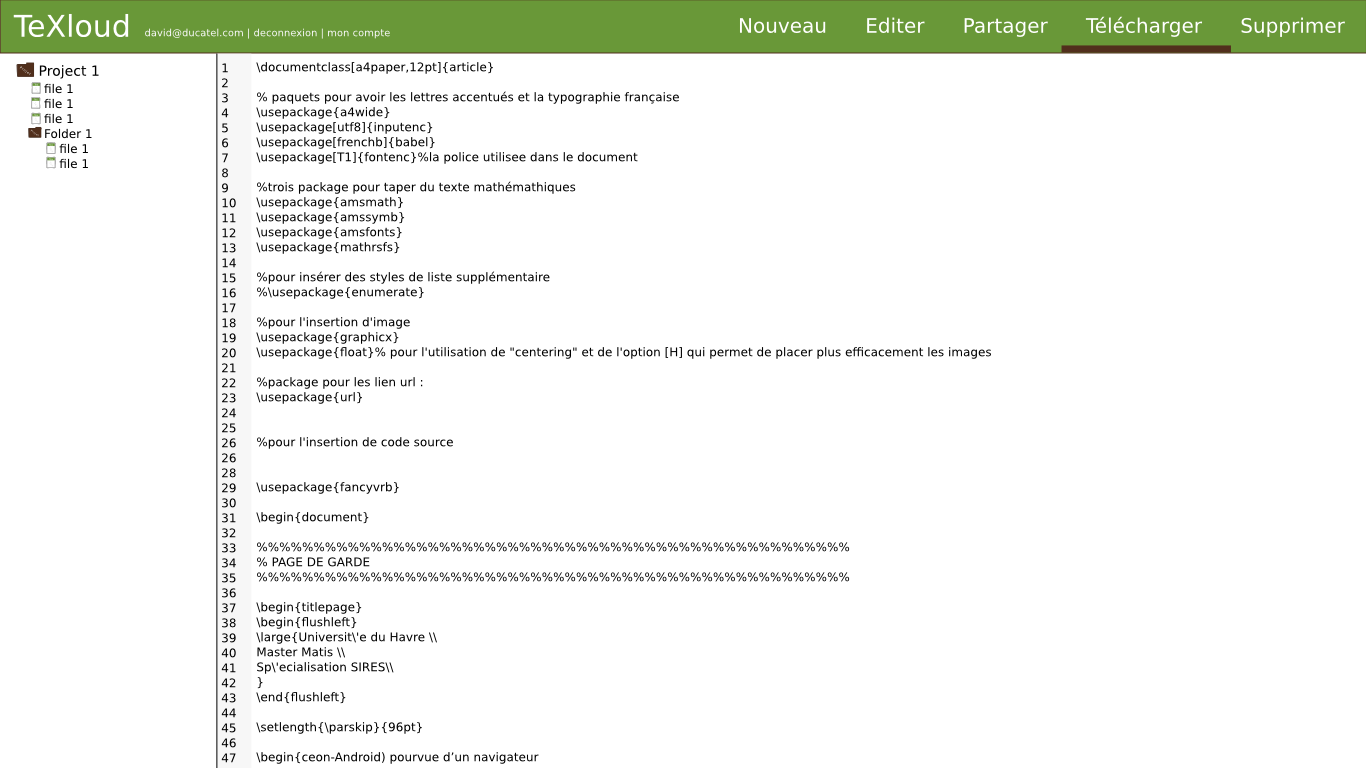
\includegraphics[width=1\textwidth, angle=90]{../layout/layout_texloud_project.png}
\end{center}
  \caption{Inteface de projet}
  \label{uiProject}
\end{figure}

\newpage
\subsubsection{Interface d'édition}
\paragraph{}
\begin{figure}[!ht]
\begin{center}
  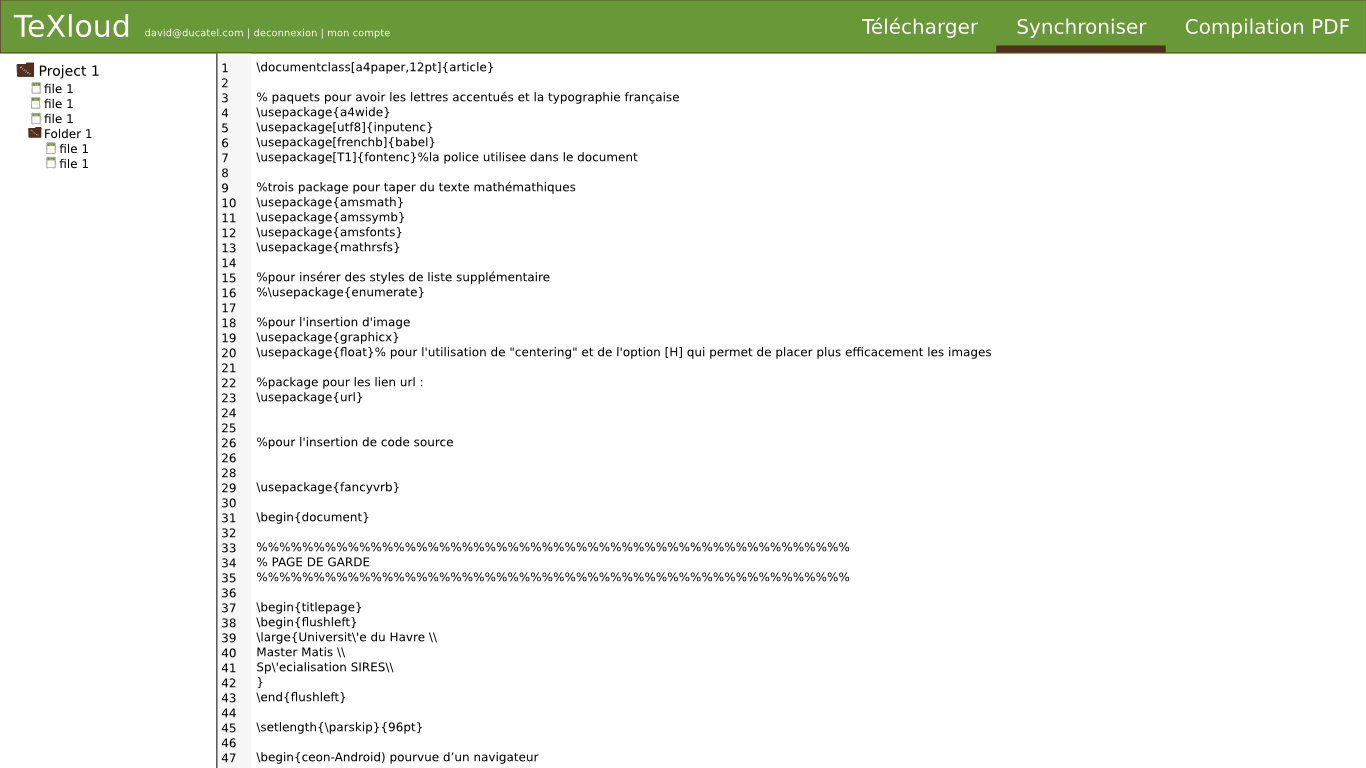
\includegraphics[width=1\textwidth, angle=90]{../layout/layout_texloud_std.png}
\end{center}
  \caption{Interface d'édition}
  \label{uiEdit}
\end{figure}

\newpage
\section{Macro-planning}
\paragraph{}
\begin{figure}[!ht]
\begin{center}
  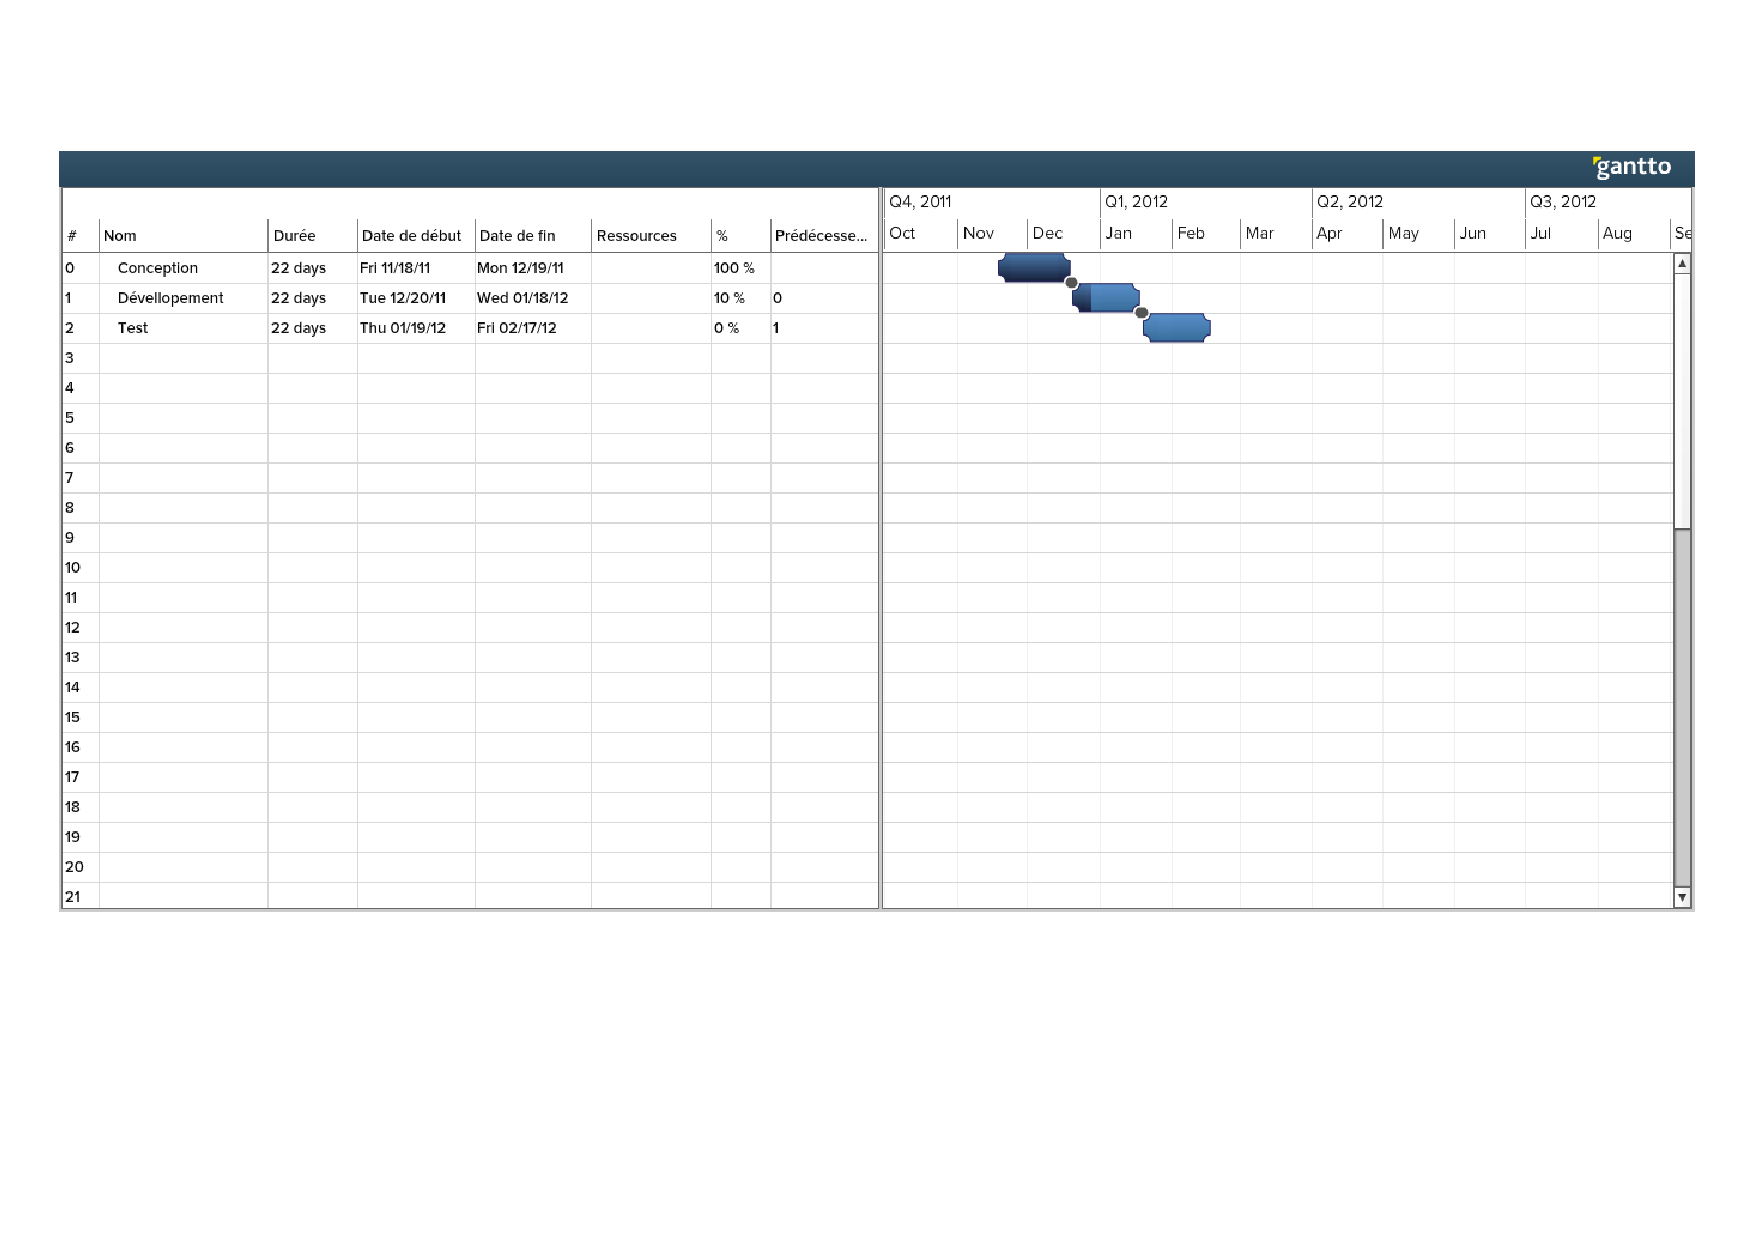
\includegraphics[width=1.1\textwidth,
angle=90]{./Ressources/macroPlanning.pdf}
\end{center}
  \caption{Macro planning}
  \label{uiProject}
\end{figure}

\newpage
\section{Matrice de Traçabilité}



\appendix
\newpage

\section{Diagramme de cas d'utilisation}
\paragraph{}
\begin{figure}[!ht]
\begin{center}
  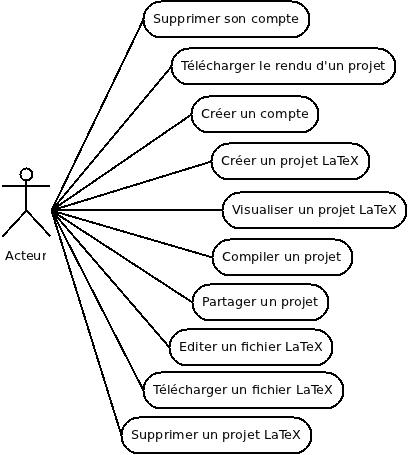
\includegraphics[width=1\textwidth]{./Diagramme/diaUseCase.jpg}
\end{center}
  \caption{Diagramme de cas d'utilisation}
  \label{useCases}
\end{figure}

\newpage
\section{Diagramme de séquences de l'interface web}
\subsubsection{Inscription}
\paragraph{}
\begin{figure}[!ht]
\begin{center}
  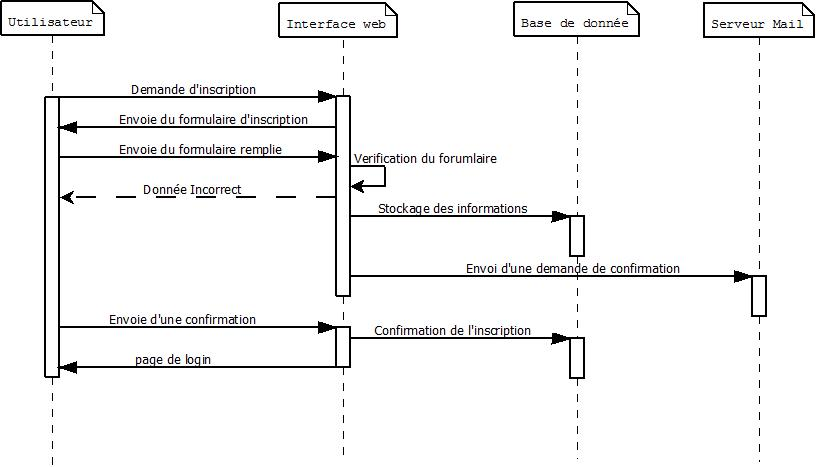
\includegraphics[width=1\textwidth, angle=90]{./Diagramme/CompteInscription.jpg}
\end{center}
  \caption{Scénario d'inscription}
  \label{register}
\end{figure}

\newpage
\subsubsection{Suppression de compte}
\paragraph{}
\begin{figure}[!ht]
\begin{center}
  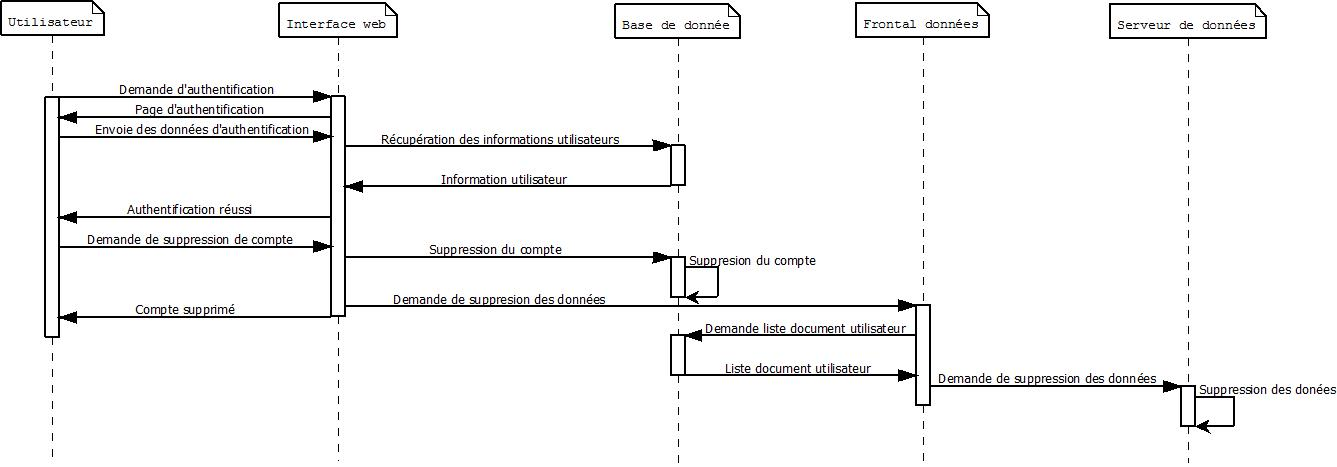
\includegraphics[width=1\textwidth, angle=90]{./Diagramme/CompteSuppression.jpg}
\end{center}
  \caption{Scénario de suppression de compte}
  \label{deleteAccount}
\end{figure}

\newpage
\subsubsection{Création d'un projet}
\paragraph{}
\begin{figure}[!ht]
\begin{center}
  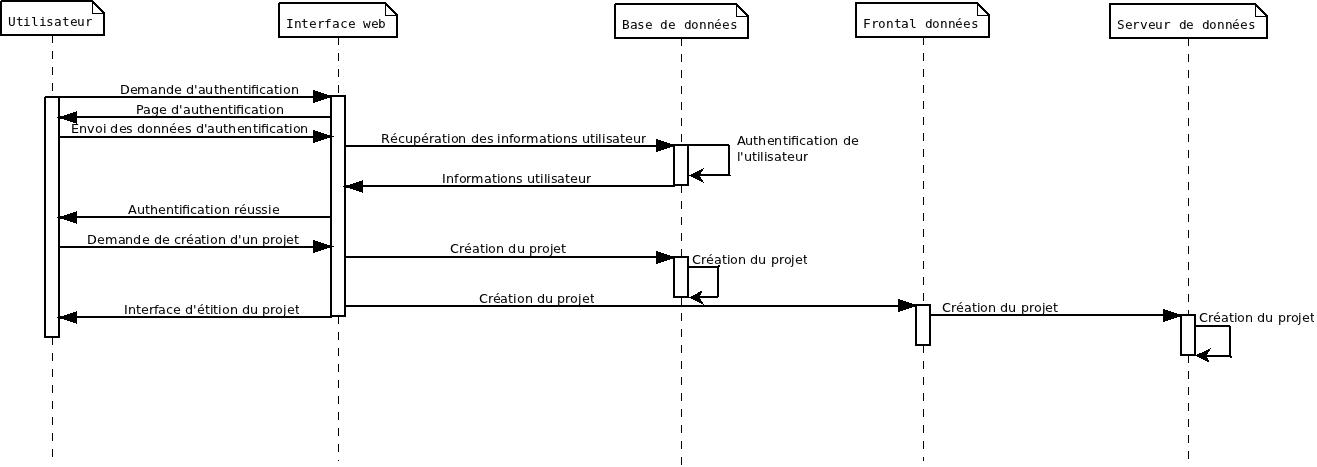
\includegraphics[width=1\textwidth, angle=90]{./Diagramme/CreationProjet.jpg}
\end{center}
  \caption{Scénario de création d'un projet}
  \label{createProject}
\end{figure}

\newpage
\subsubsection{Compilation de documents}
\paragraph{}
\begin{figure}[!ht]
\begin{center}
  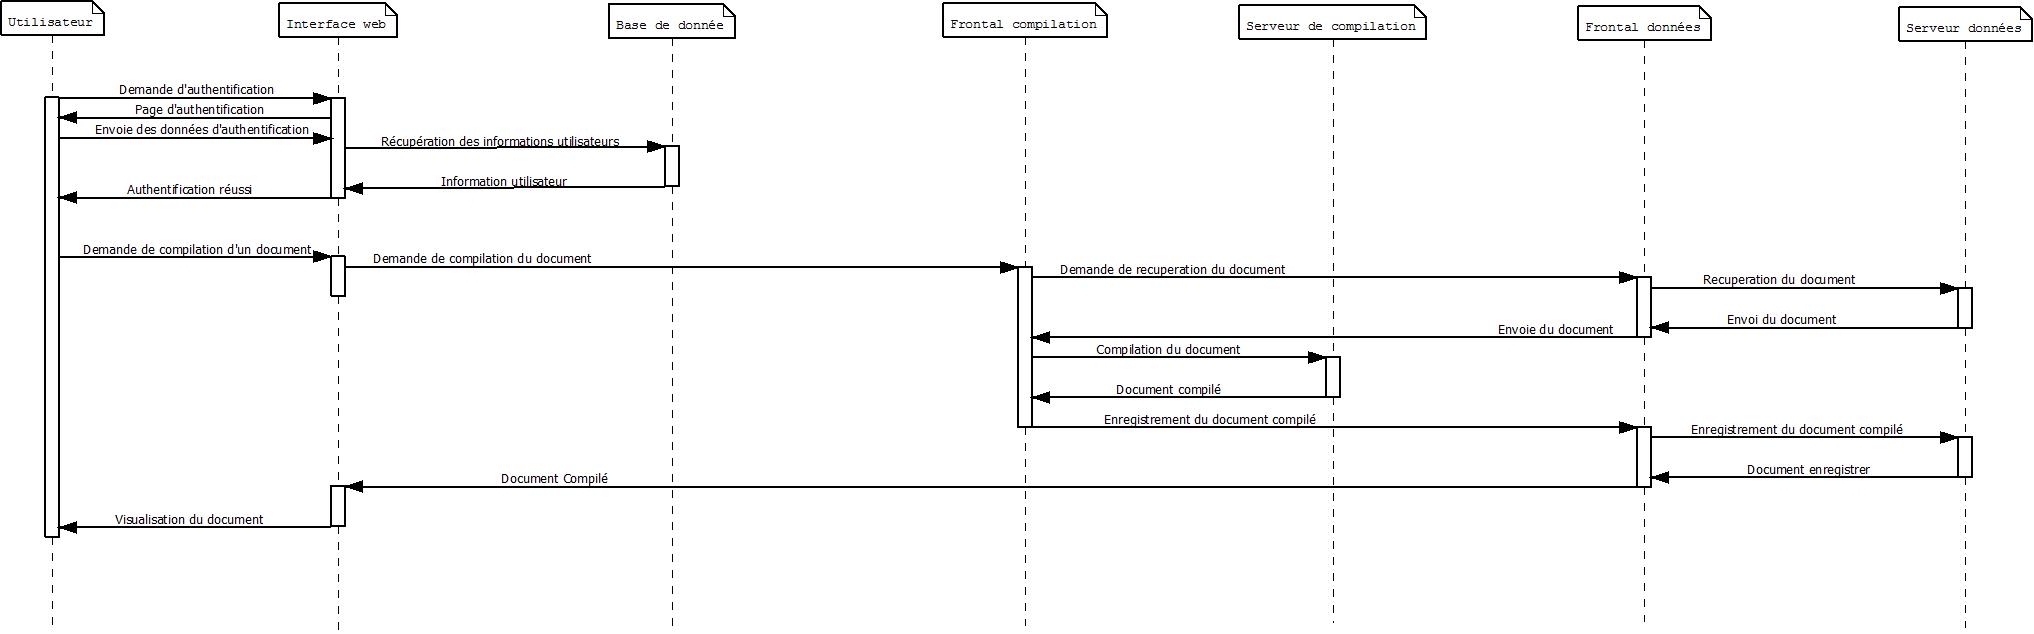
\includegraphics[width=1\textwidth, angle=90]{./Diagramme/DemandeCompilation.jpg}
\end{center}
  \caption{Scénario de compilation de document}
  \label{compile}
\end{figure}

\newpage
\subsubsection{Téléchargement de fichiers}
\paragraph{}
\begin{figure}[!ht]
\begin{center}
  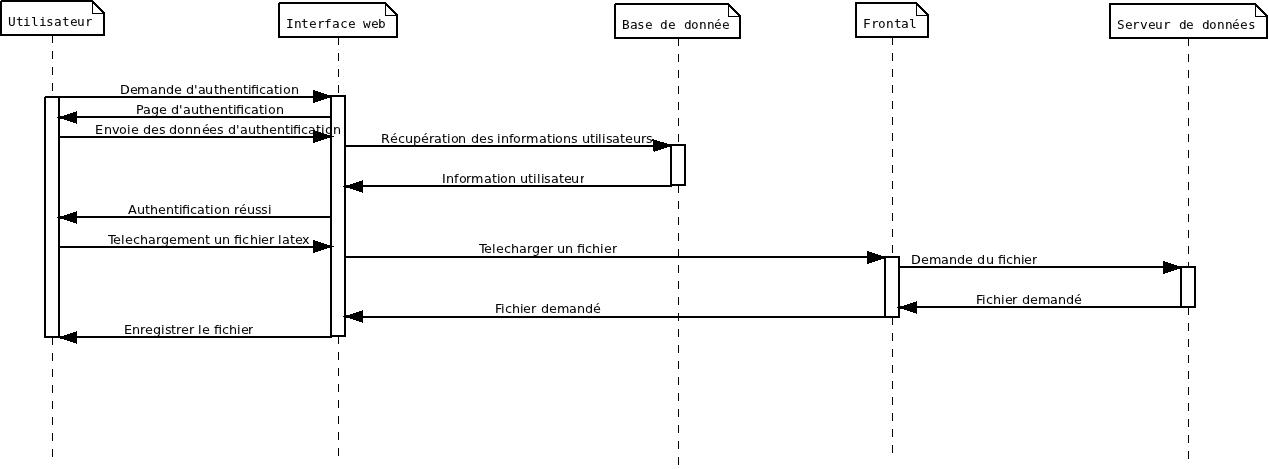
\includegraphics[width=1\textwidth, angle=90]{./Diagramme/FichierLatexTelechargement.jpg}
\end{center}
  \caption{Scénario de téléchargement de document}
  \label{download}
\end{figure}

\newpage
\subsubsection{Partage de projet}
\paragraph{}
\begin{figure}[!ht]
\begin{center}
  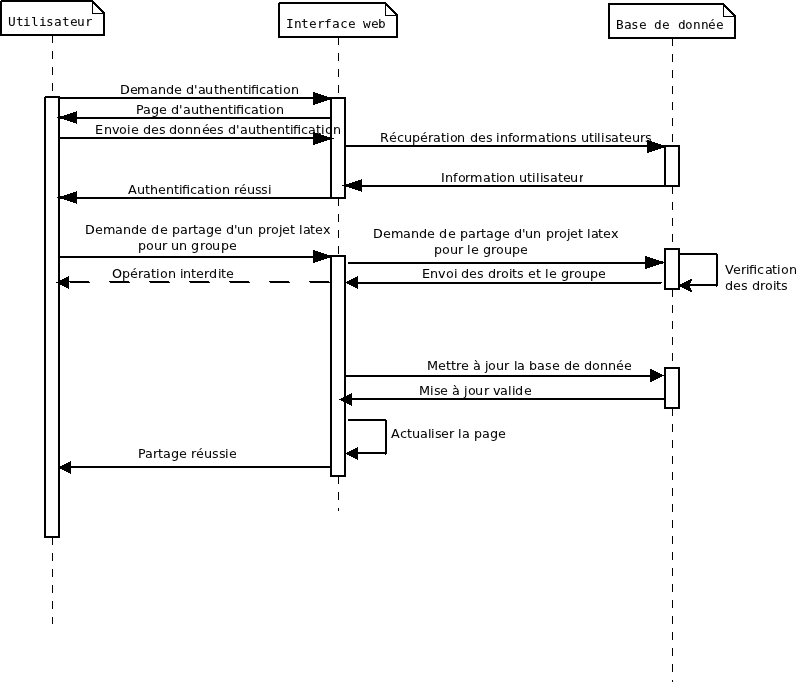
\includegraphics[width=1\textwidth, angle=90]{./Diagramme/PartageProjet.png}
\end{center}
  \caption{Scénario de partage d'un projet}
  \label{share}
\end{figure}

\newpage
\subsubsection{Synchronisation de documents}
\paragraph{}
\begin{figure}[!ht]
\begin{center}
  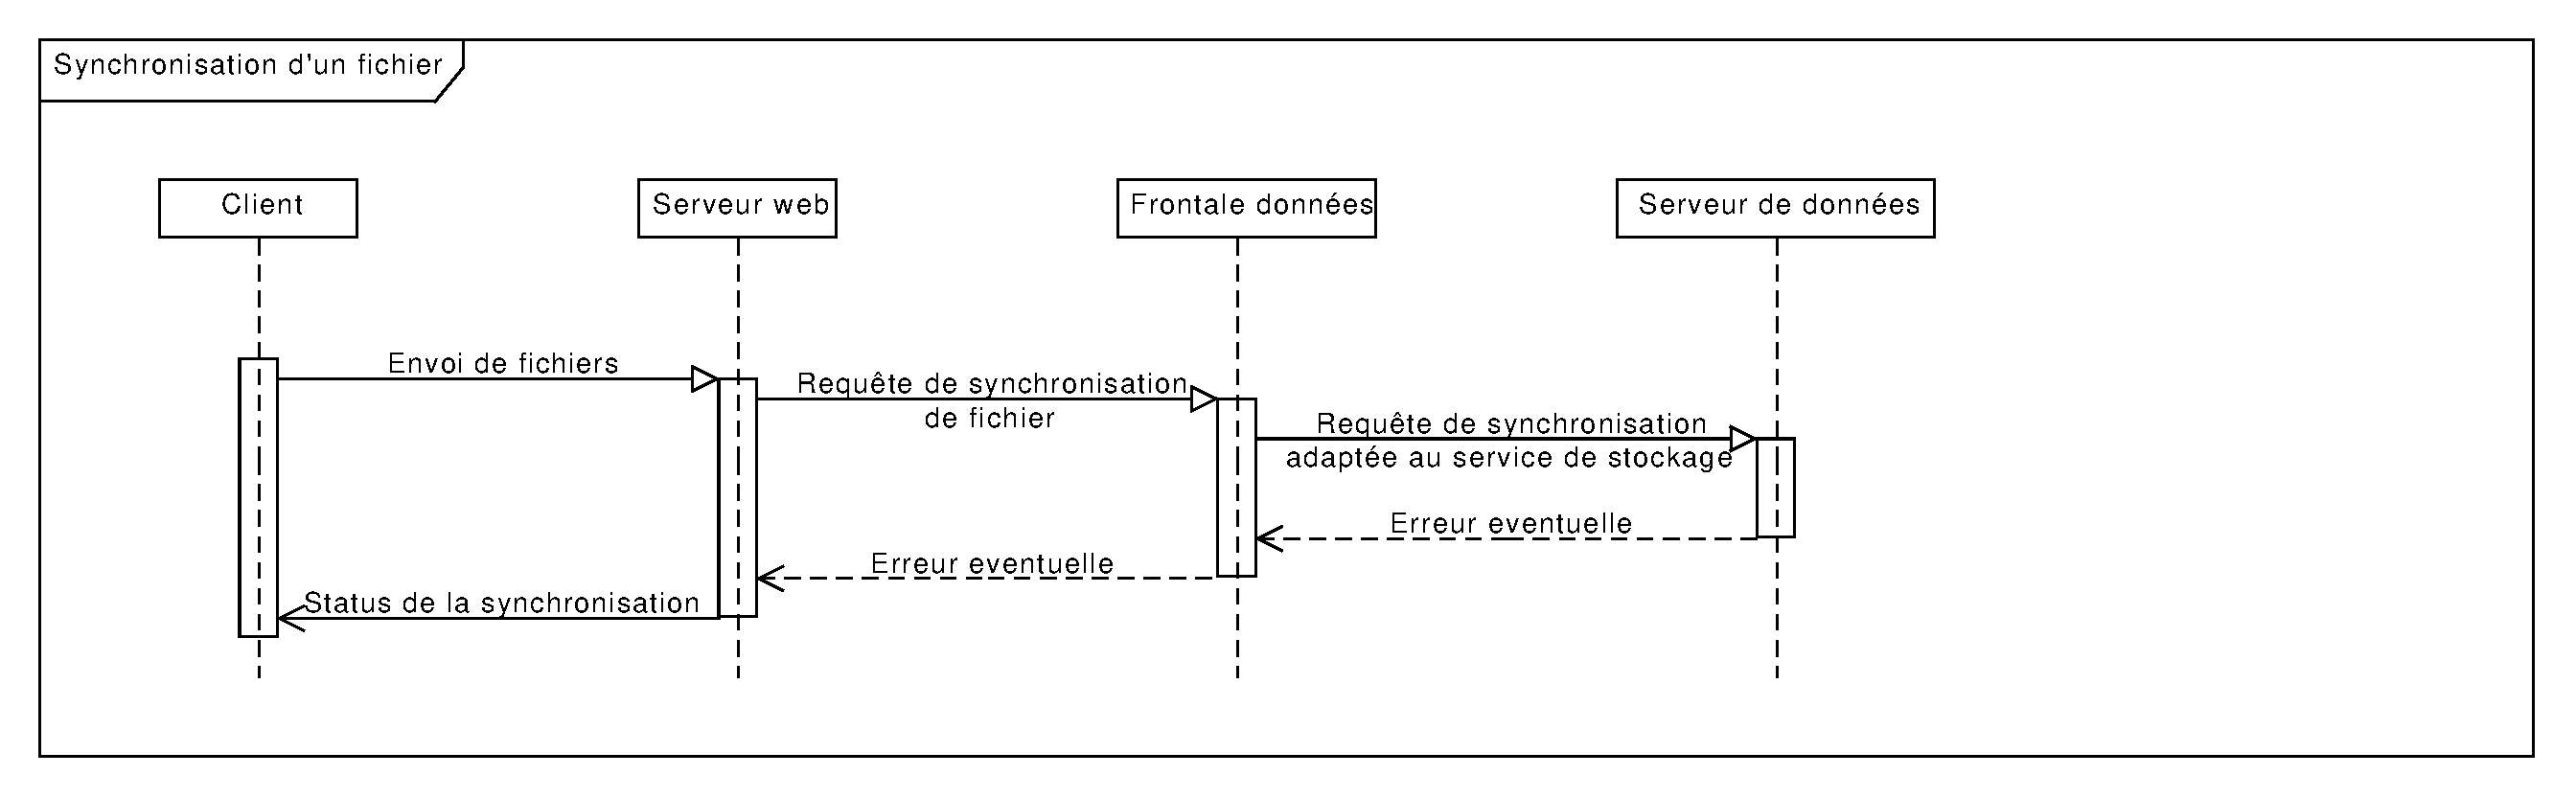
\includegraphics[width=1\textwidth, angle=90]{./Diagramme/data_sync.pdf}
\end{center}
  \caption{Scénario de synchronisation de documents}
  \label{sync}
\end{figure}

\newpage
\subsubsection{Visualisation d'un projet}
\paragraph{}
\begin{figure}[!ht]
\begin{center}
  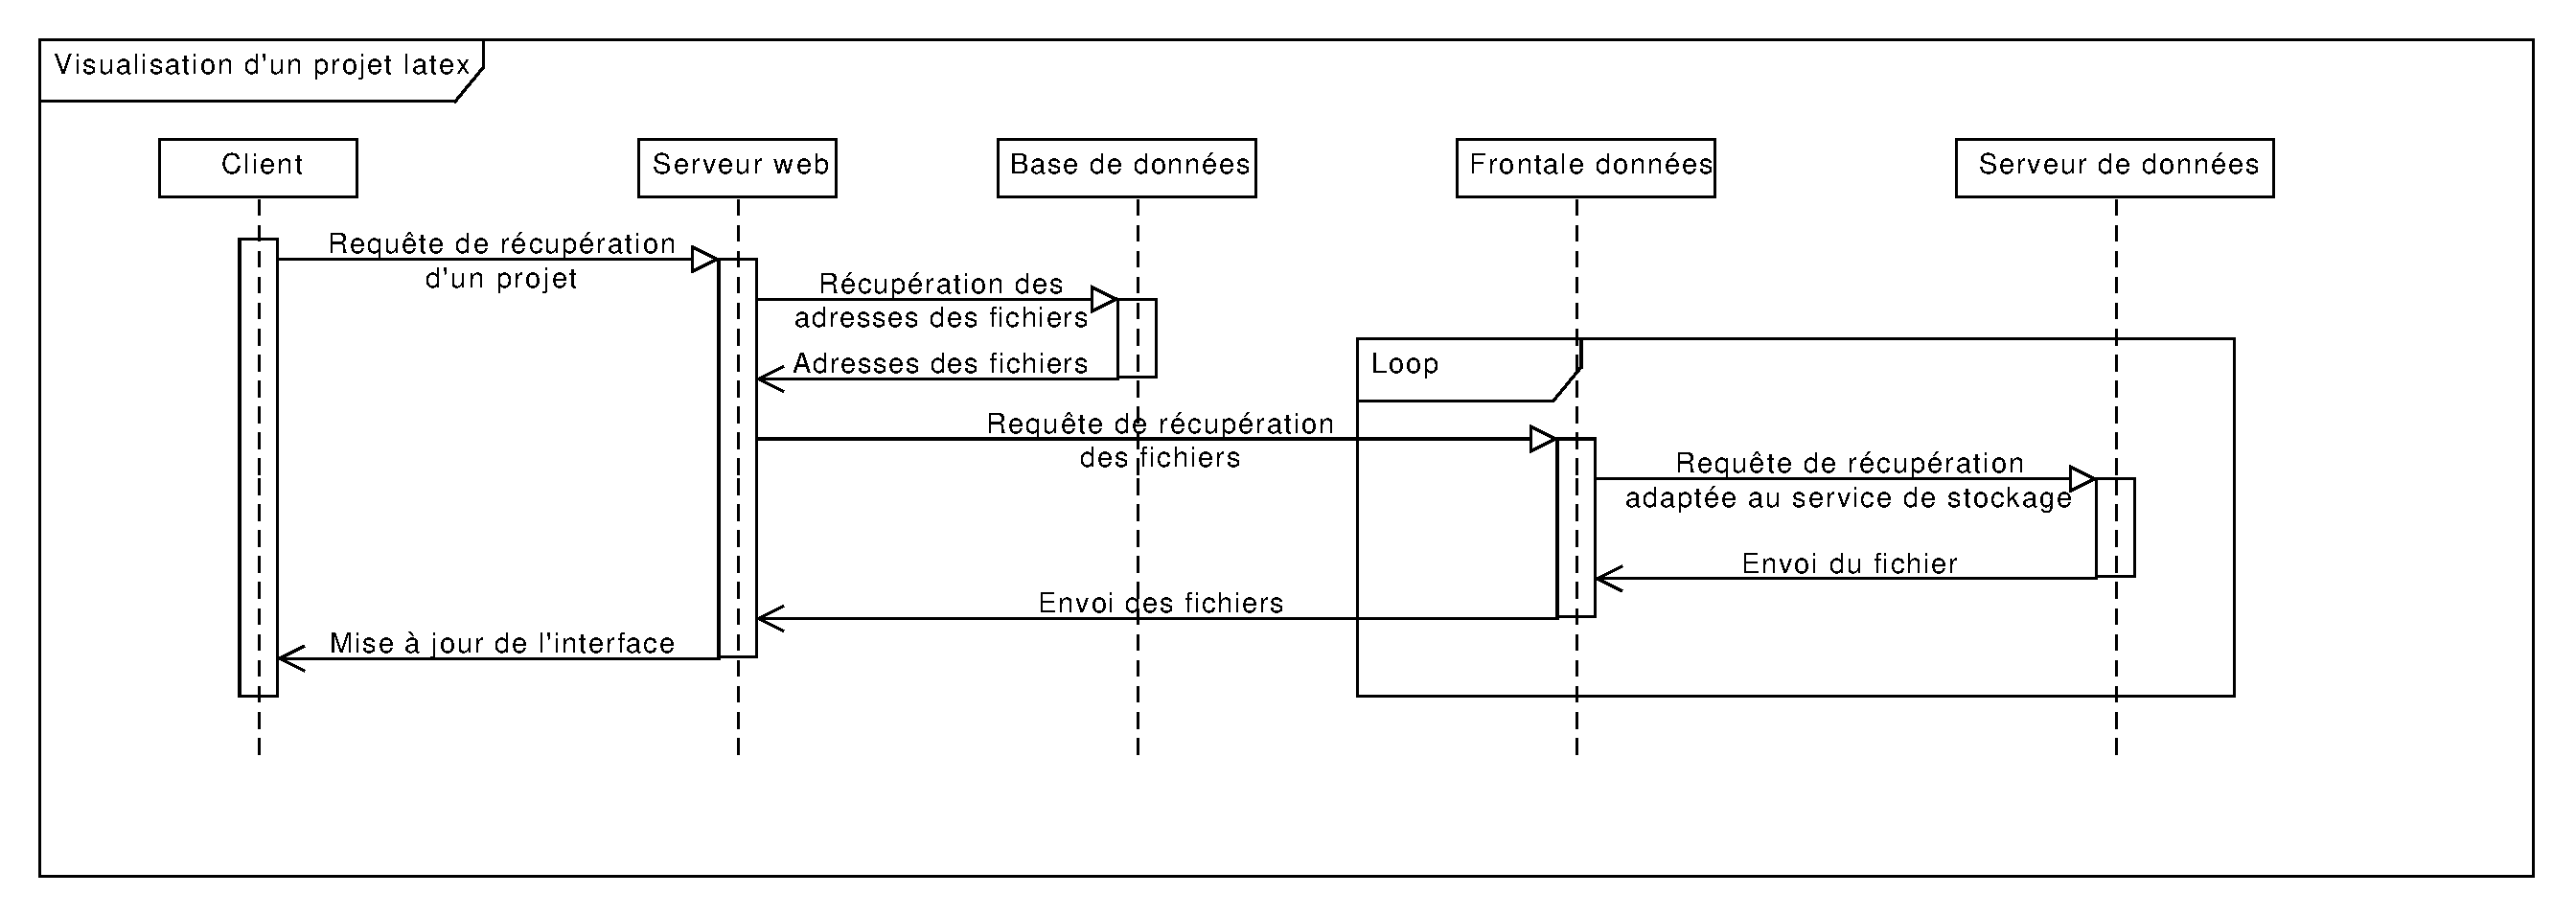
\includegraphics[width=1\textwidth, angle=90]{./Diagramme/project_visu.pdf}
\end{center}
  \caption{Scénario de visualisation d'un projet}
  \label{view}
\end{figure}

\newpage
\subsubsection{Suppression d'un projet}
\paragraph{}
\begin{figure}[!ht]
\begin{center}
  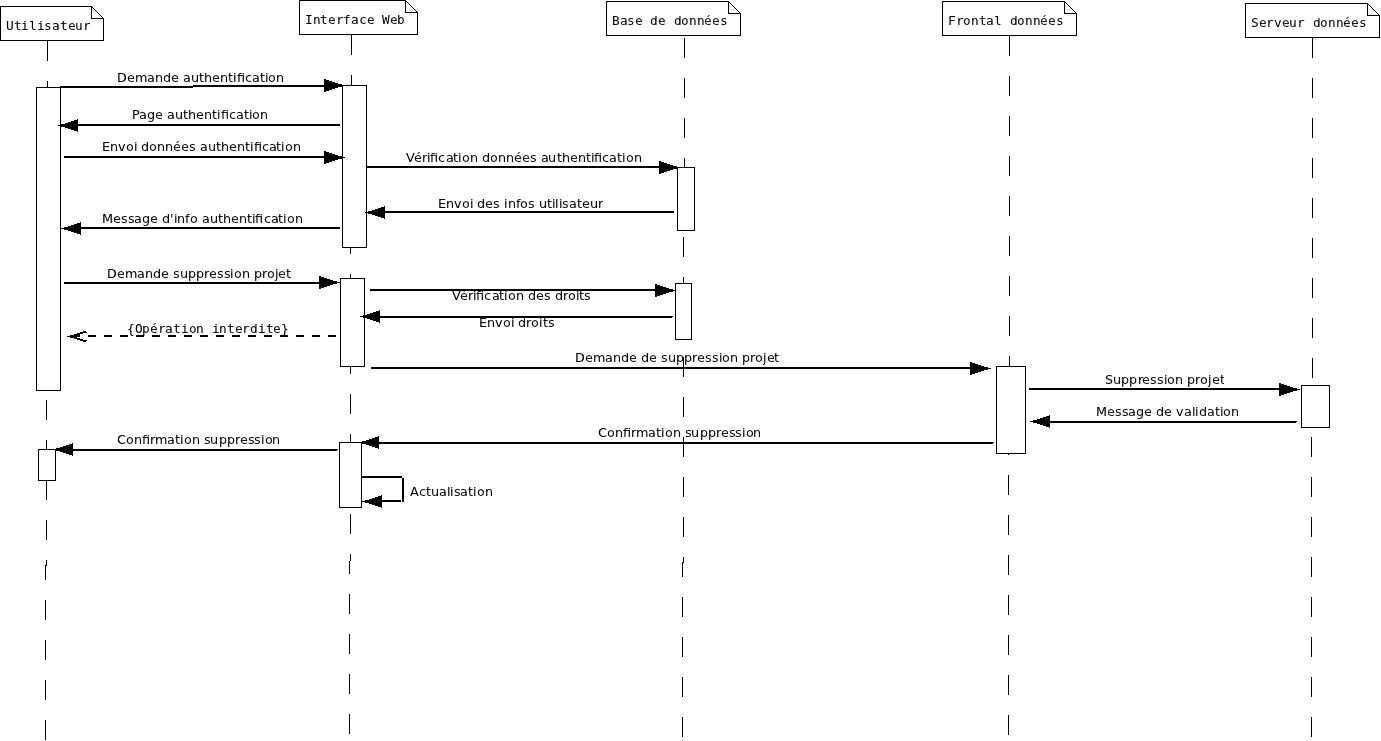
\includegraphics[width=1\textwidth, angle=90]{./Diagramme/SuppressionProjetViaWeb.jpg}
\end{center}
  \caption{Scénario de suppression d'un projet}
  \label{deleteProject}
\end{figure}

\newpage
\subsubsection{Téléchargement d'un projet}
\paragraph{}
\begin{figure}[!ht]
\begin{center}
  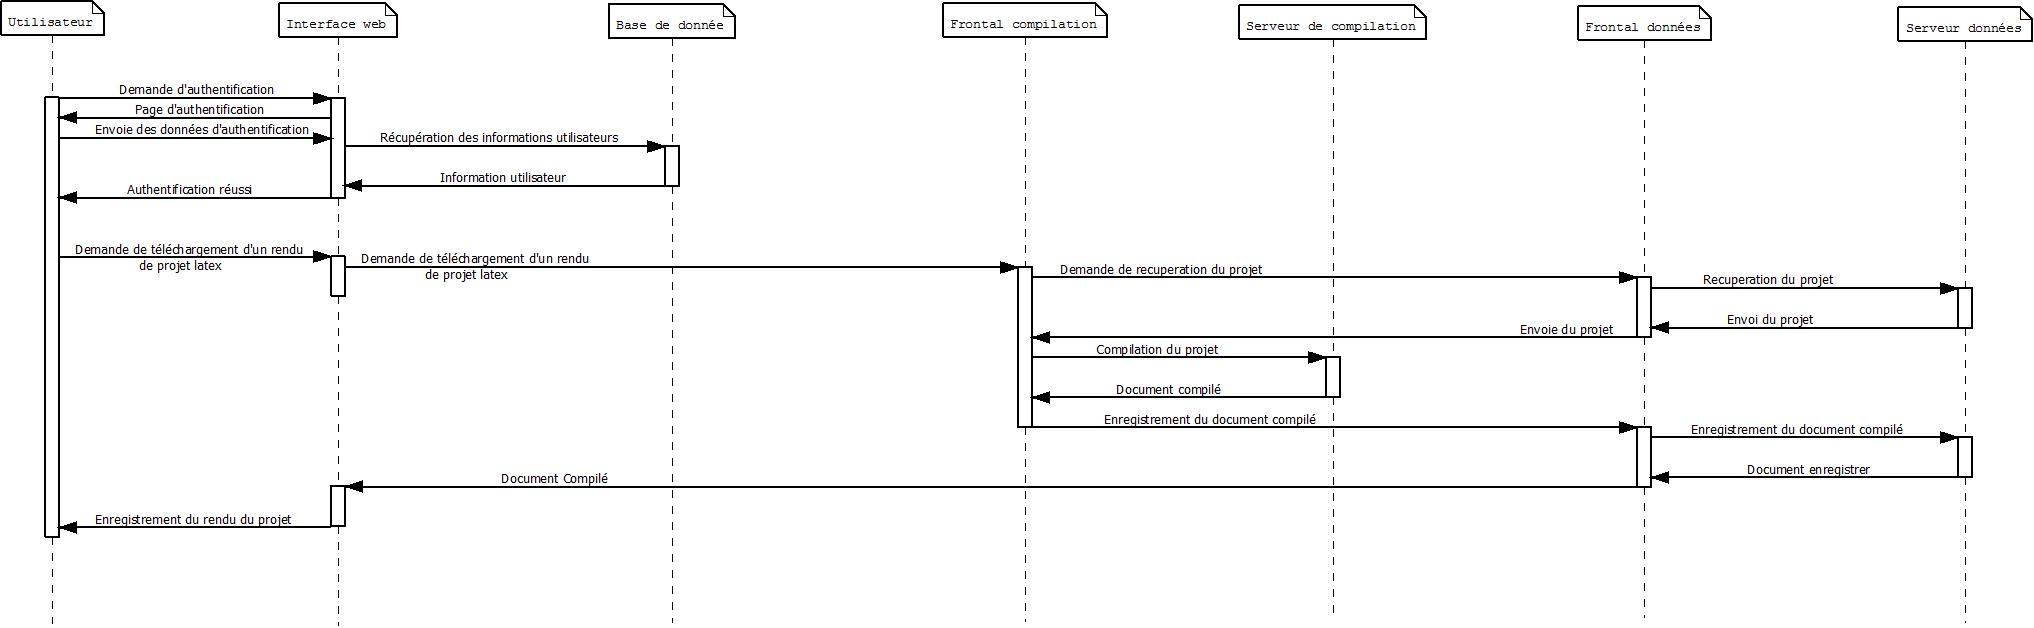
\includegraphics[width=1\textwidth, angle=90]{./Diagramme/telechargementRenduProjet.jpg}
\end{center}
  \caption{Scénario de téléchargement d'un projet}
  \label{downloadProject}
\end{figure}

\section{Diagramme de séquences de l'application Android}
\subsubsection{Inscription}
\paragraph{}
\begin{figure}[!ht]
\begin{center}
  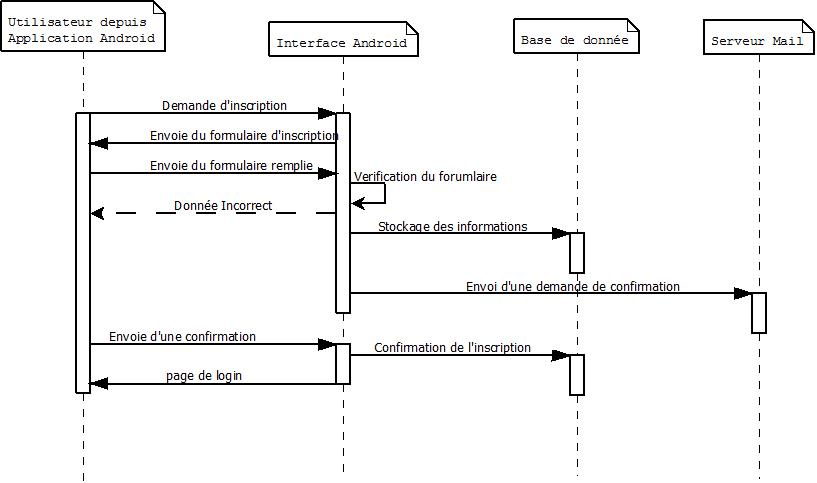
\includegraphics[width=1\textwidth, angle=90]{./Diagramme/Android/CompteInscription.jpg}
\end{center}
  \caption{Scénario d'inscription}
  \label{androidRegister}
\end{figure}

\newpage
\subsubsection{Suppression de compte}
\paragraph{}
\begin{figure}[!ht]
\begin{center}
  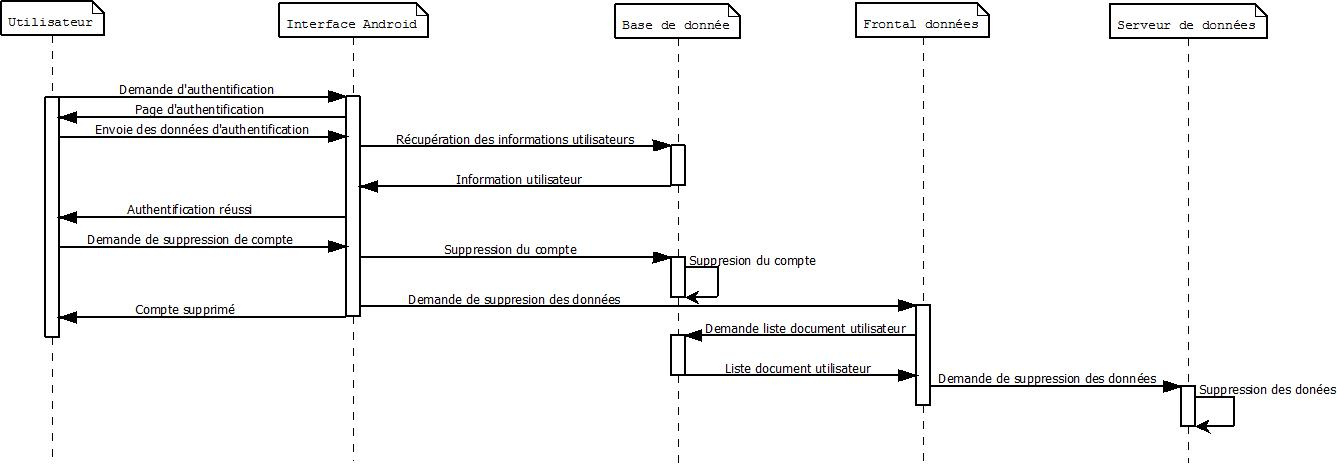
\includegraphics[width=1\textwidth, angle=90]{./Diagramme/Android/CompteSuppression.jpg}
\end{center}
  \caption{Scénario de suppression de compte}
  \label{androidDeleteAccount}
\end{figure}

\newpage
\subsubsection{Création de projet}
\paragraph{}
\begin{figure}[!ht]
\begin{center}
  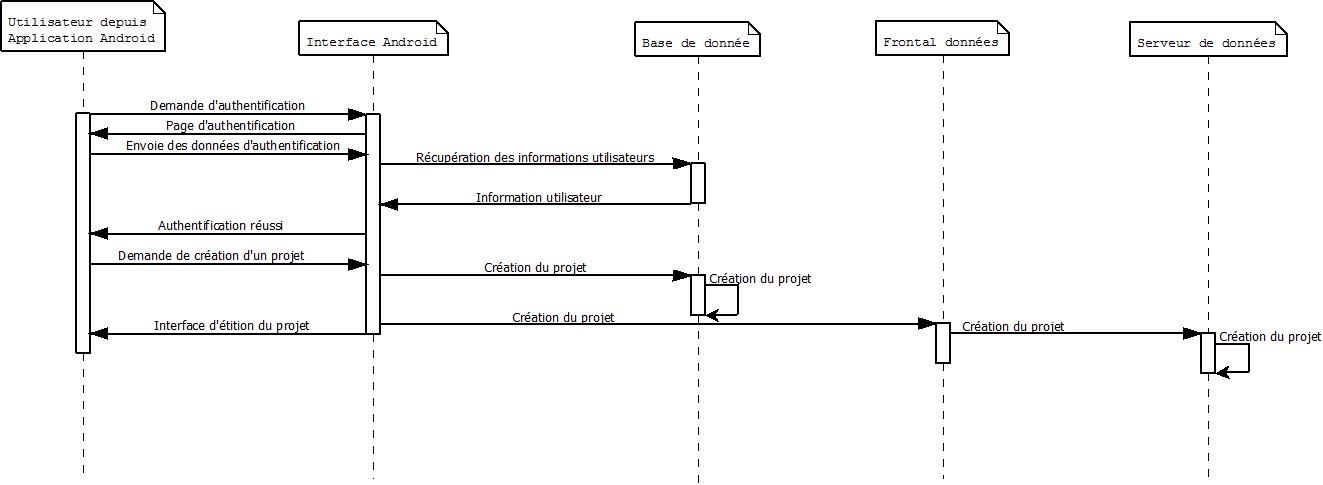
\includegraphics[width=1\textwidth, angle=90]{./Diagramme/Android/CreationProjet.jpg}
\end{center}
  \caption{Scénario de Création de projet}
  \label{androidCreateProject}
\end{figure}

\newpage
\subsubsection{Compilation de documents}
\paragraph{}
\begin{figure}[!ht]
\begin{center}
  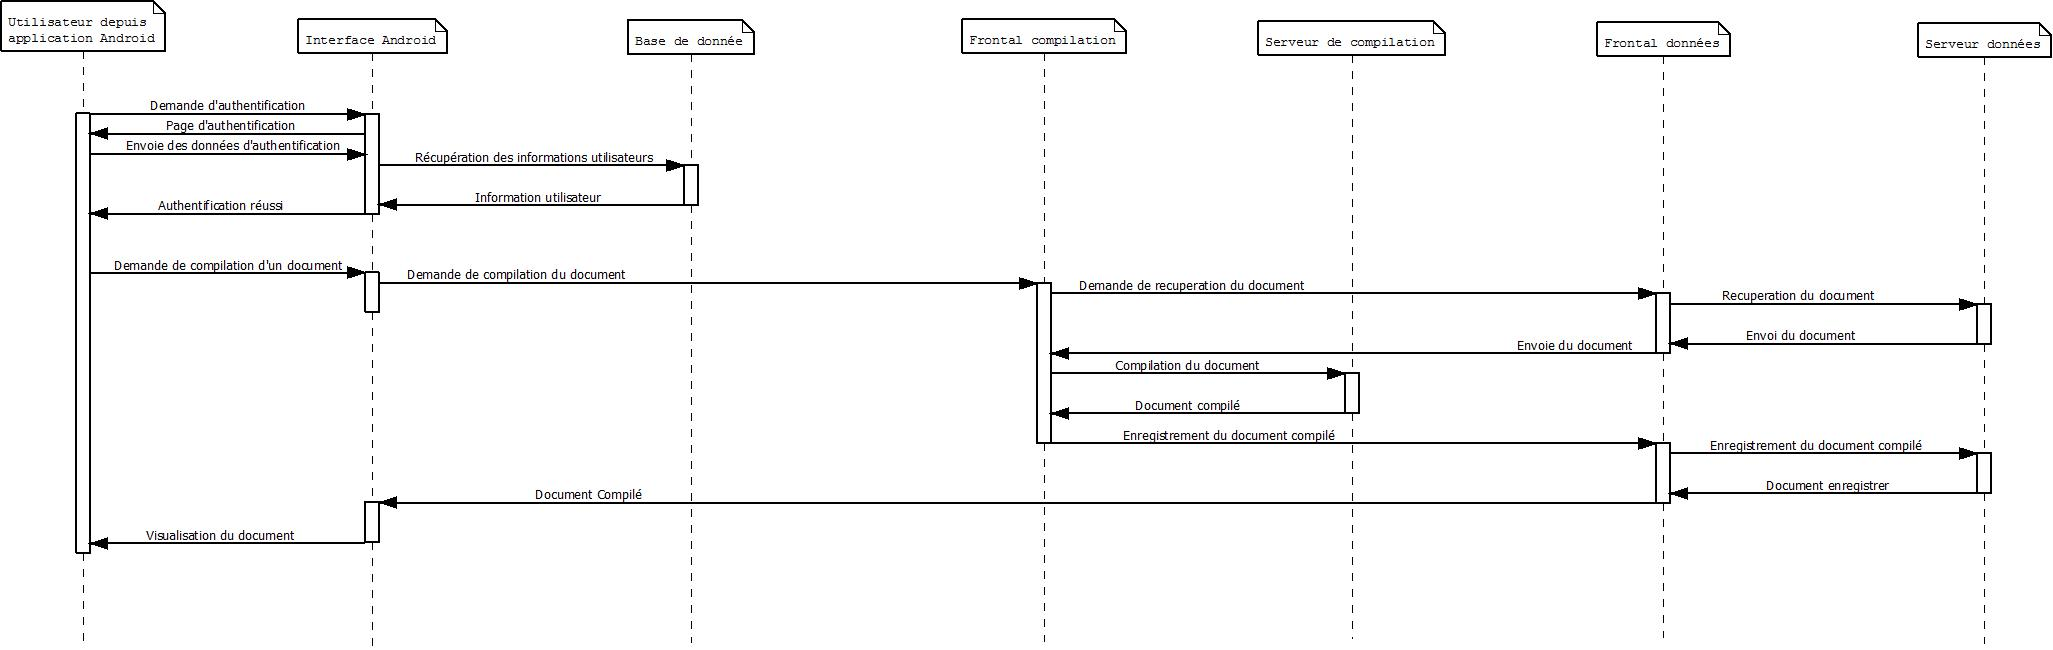
\includegraphics[width=1\textwidth, angle=90]{./Diagramme/Android/DemandeCompilation.jpg}
\end{center}
  \caption{Scénario de compilation de documents}
  \label{androidCompile}
\end{figure}

\newpage
\subsubsection{Téléchargement de documents}
\paragraph{}
\begin{figure}[!ht]
\begin{center}
  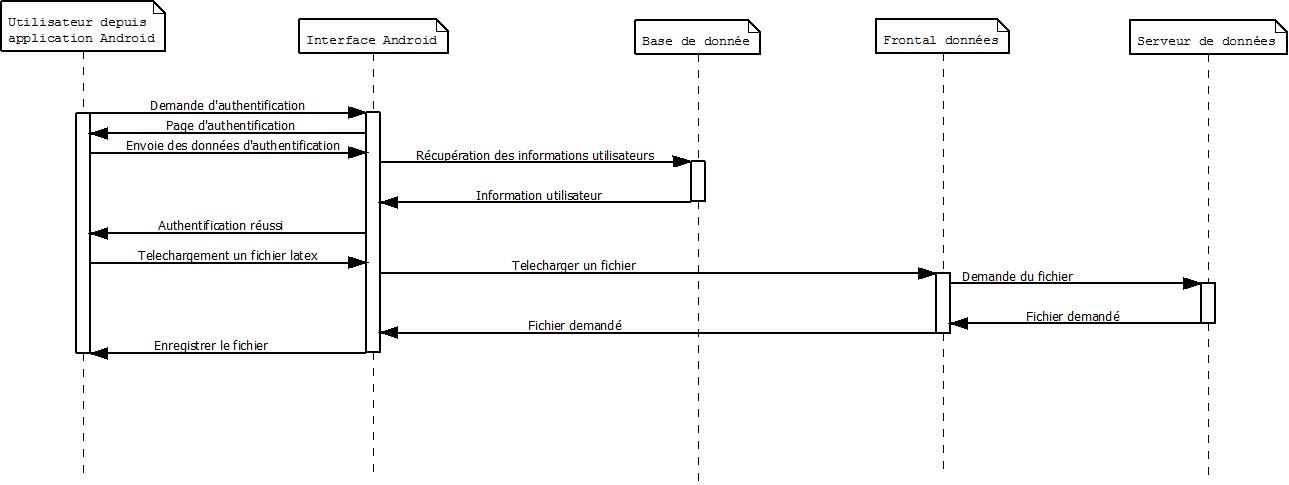
\includegraphics[width=1\textwidth, angle=90]{./Diagramme/Android/FichierLatexTelechargement.jpg}
\end{center}
  \caption{Scénario de téléchargement de documents}
  \label{androidDownload}
\end{figure}

\newpage
\subsubsection{Suppression d'un projet}
\paragraph{}
\begin{figure}[!ht]
\begin{center}
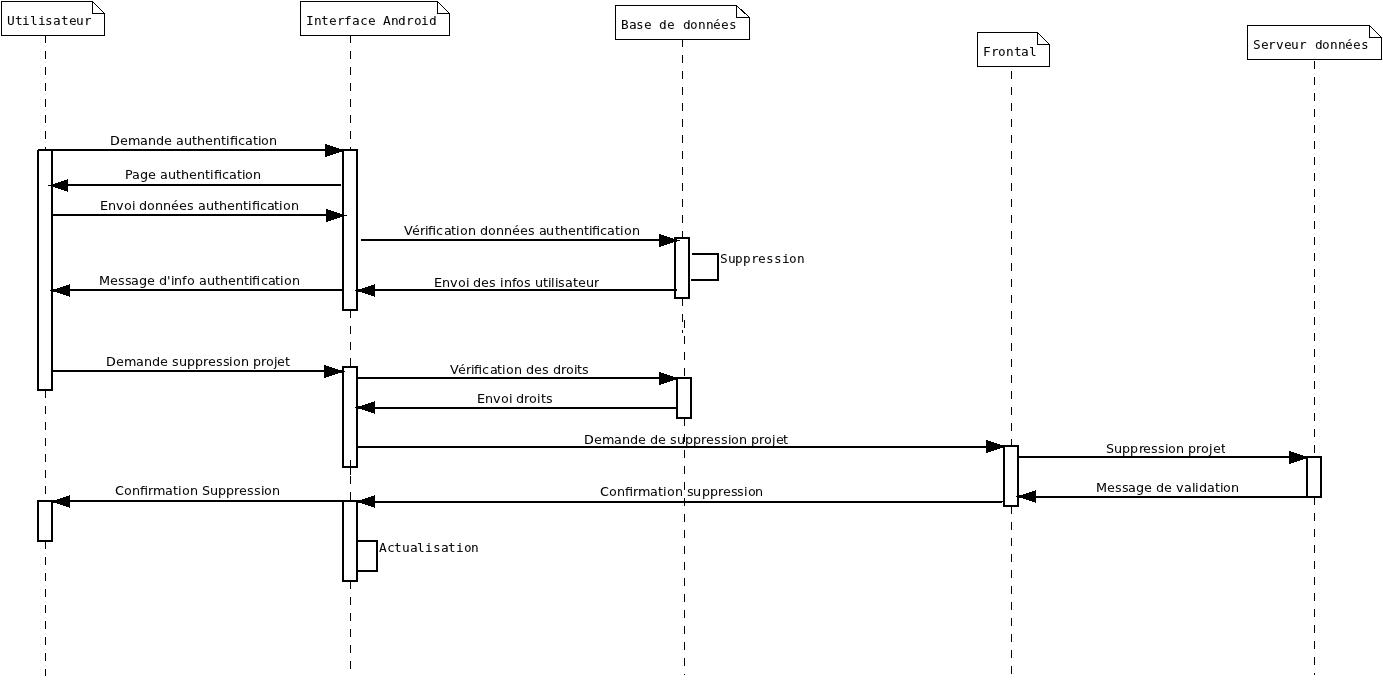
\includegraphics[width=1\textwidth,angle=90]{
./Diagramme/Android/SuppressionProjetViaAndroid.jpg}
\end{center}
  \caption{Scénario de suppression d'un projet}
  \label{androidDel}
\end{figure}

\newpage
\subsubsection{Téléchargement d'un projet}
\paragraph{}
\begin{figure}[!ht]
\begin{center}
  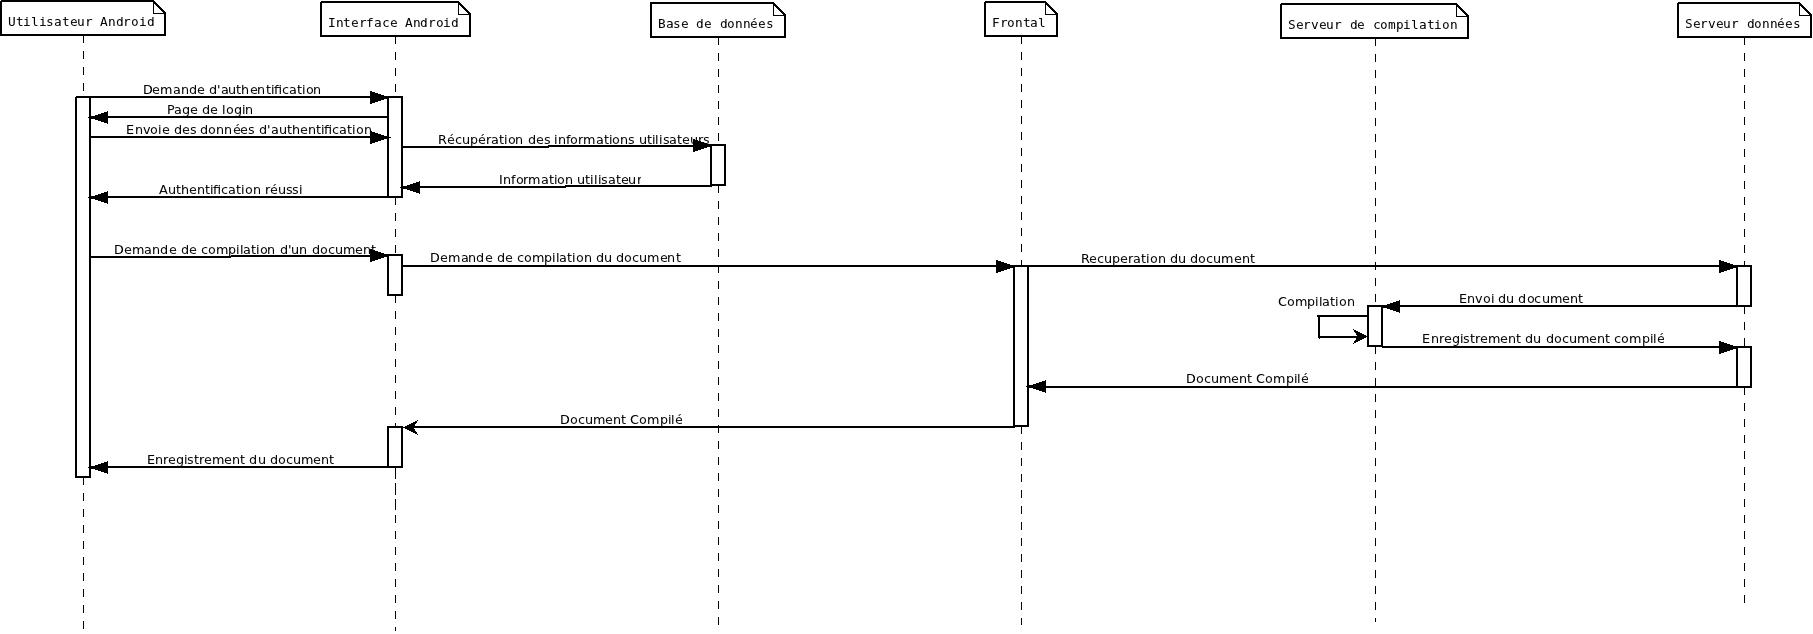
\includegraphics[width=1\textwidth, angle=90]{./Diagramme/Android/telechargementRenduProjet.jpg}
\end{center}
  \caption{Scénario de téléchargement d'un projet}
  \label{androidDownloadProject}
\end{figure}

\newpage
\listoffigures
\end{document}
